\documentclass[12pt,titlepage]{article}
\usepackage[margin=1.25in]{geometry}
\usepackage{graphicx,amsmath,blindtext,enumitem,minted,multicol,tabularx}

%% Variables definition
\newcommand{\vSubject}{Information Technology Concepts}
\newcommand{\vSubtitle}{Jobsheet 6}
\newcommand{\vName}{Dicha Zelianivan Arkana}
\newcommand{\vNIM}{2241720002}
\newcommand{\vClass}{1i}
\newcommand{\vDepartment}{Information Technology}
\newcommand{\vStudyProgram}{D4 Informatics Engineering}

%% [START] Tikz related stuff
\usepackage{tikz}
\usetikzlibrary{svg.path,calc,shapes.geometric,shapes.misc}
\tikzstyle{terminator} = [rectangle, draw, text centered, rounded corners = 1em, minimum height=2em]
\tikzstyle{preparation} = [chamfered rectangle, chamfered rectangle sep=0.75em, draw, text centered, minimum height = 2em]
\tikzstyle{process} = [rectangle, draw, text centered, minimum height=2em]
\tikzstyle{decision} = [diamond, aspect=2, draw, text centered, minimum height=2em]
\tikzstyle{data}=[trapezium, draw, text centered, trapezium left angle=60, trapezium right angle=120, minimum height=2em]
\tikzstyle{connector} = [line width=0.25mm,->]
%% [END] Tikz related stuff

%% [START] Fancy header related stuff
\usepackage{fancyhdr}
\pagestyle{fancy}
\setlength{\headheight}{15pt} % compensate fancyhdr style
\fancyhead{}
\fancyfoot{}
\fancyfoot[L]{\thepage}
\fancyfoot[R]{\textit{\vSubject - \vSubtitle}}
\renewcommand{\footrulewidth}{0.4pt}% default is 0pt, overline for footer
%% [END] Fancy header related stuff

%% [START] Custom tabular command related stuff
\usepackage{tabularx}
\newcommand{\details}[2]{
    #1 & #2  \\
}
%% [END] Custom tabular command related stuff

%% [START] Figure related stuff
\newcommand{\image}[3][1]{
    \begin{figure}[h]
        \centering
        \includegraphics[#1]{#2}
        \caption{#3}
        \label{#3}
    \end{figure}
}
%% [END] Figure related stuff

\begin{document}
\begin{titlepage}
    \centering
    \vfill
    {\bfseries\LARGE
        \vSubject\\
        \vskip0.25cm
        \vSubtitle
    }
    \vfill
    
\includegraphics[width=6cm]{images/polinema-logo.png}
    \vfill
    {
        \textbf{Name}\\
        \vName\\
        \vskip0.5cm
        \textbf{NIM}\\
        \vNIM\\
        \vskip0.5cm
        \textbf{Class}\\
        \vClass\\
        \vskip0.5cm
        \textbf{Department}\\
        \vDepartment\\
        \vskip0.5cm
        \textbf{Study Program}\\
        \vStudyProgram
    }
\end{titlepage}

\tableofcontents
\pagebreak

\section{Laboratory}
\subsection{Experiment 1: Calculate factorial values using iteration}
\begin{enumerate}[label=\alph*)]
    \item {
        Loop using \textbf{for}

        \begin{enumerate}[label=\arabic*.]
            \item Open a text editor. Create a new file, name it \textbf{FactorialFor.java}
            \item Write the basic structure of Java programming language which contains the \texttt{main()} function.
            \item Add the Scanner library
            \item Make a \textbf{Scanner} declaration with the name \texttt{input}
            \item Create multiple \texttt{int} type variables with names \texttt{number}, \texttt{factorial}, and \texttt{i}
            \item {
                Write down the syntax for entering the value from keyboard

                \begin{minted}[autogobble,fontsize=\small]{java}
                    System.out.print("Enter a number: ");
                    number = input.nextInt();
                \end{minted}
            }
            \pagebreak
            \item {
                Create a for loop structure to calculate the factorial

                \begin{minted}[autogobble,fontsize=\small]{java}
                    factorial = 1;
                    for (i = 1; i <= number; i++) {
                        factorial = factorial * i;
                    }
                \end{minted}
            }
            \item {
                Display factorial calculation result

                \begin{minted}[autogobble,fontsize=\small]{java}
                    System.out.printf("The factorial of %d is %d\n", number, factorial);
                \end{minted}
            }
            \item {
                Compile and run the program. Observe the results!

                \begin{figure}[h]
                    \centering
                    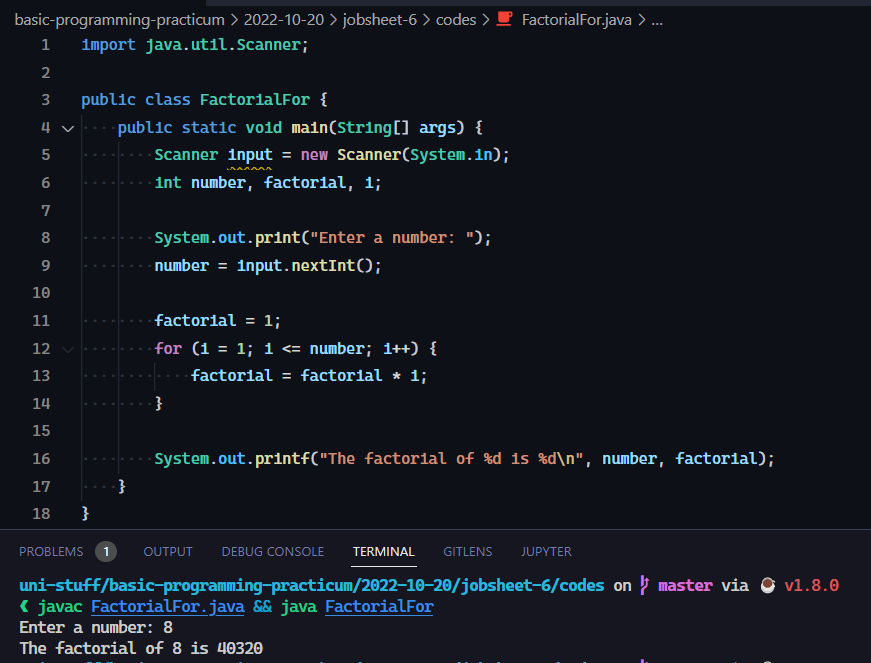
\includegraphics[width=.9\textwidth]{./images/factorial-for.png}
                    \caption{\texttt{FactorialFor.java} final code and output}
                \end{figure}
            }
        \end{enumerate}
    }
    \item {
        Loop using \textbf{while}
        \begin{enumerate}[label=\arabic*.]
            \item Open a text editor. Create a new file, name it \textbf{FactorialWhile.java}
            \item Write the basic structure of Java programming language which contains the \texttt{main()} function.
            \item Add the Scanner library
            \item Make a \textbf{Scanner} declaration with the name \texttt{input}
            \item Create multiple \texttt{int} type variables with names \texttt{number}, \texttt{factorial}, and \texttt{i}
            \item {
                Write down the syntax for entering the value from keyboard

                \begin{minted}[autogobble,fontsize=\small]{java}
                    System.out.print("Enter a number: ");
                    number = input.nextInt();
                \end{minted}
            }
            \item {
                Create a while loop structure to calculate the factorial

                \begin{minted}[autogobble,fontsize=\small]{java}
                    factorial = 1;
                    i = 1;
                    while (i <= number) {
                        factorial = factorial * i;
                        i++;
                    }
                \end{minted}
            }
            \item {
                Display factorial calculation result

                \begin{minted}[autogobble,fontsize=\small]{java}
                    System.out.printf("The factorial of %d is %d\n", number, factorial);
                \end{minted}
            }
            \item {
                Compile and run the program. Observe the results!

                \begin{figure}[h]
                    \centering
                    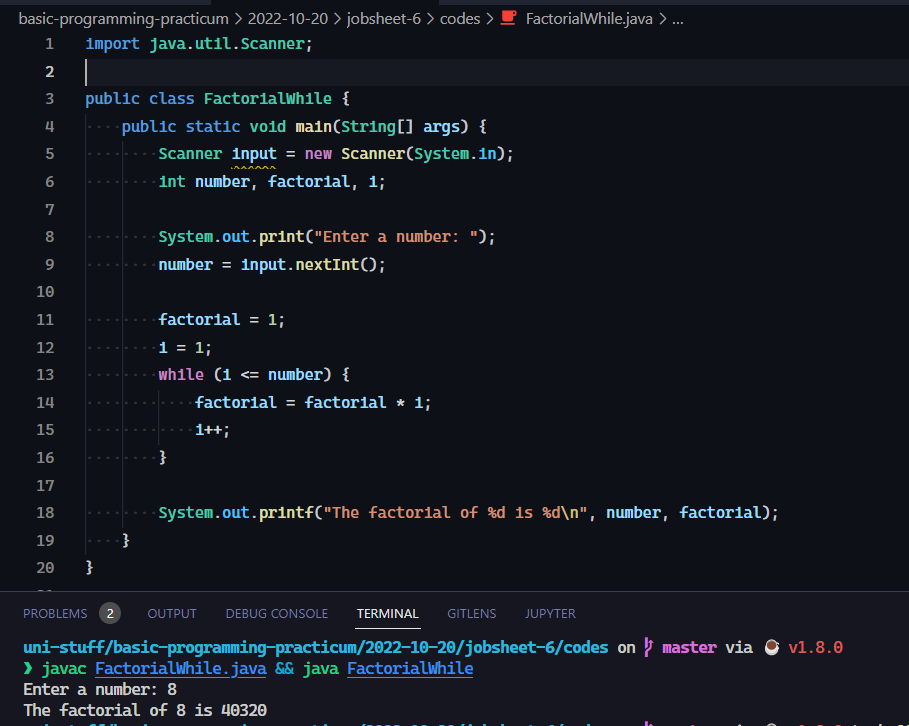
\includegraphics[width=.9\textwidth]{./images/factorial-while.png}
                    \caption{\texttt{FactorialWhile.java} final code and output}
                \end{figure}
            }
        \end{enumerate}
    }
    \pagebreak
    \item {
        Loop using \textbf{do-while}

        \begin{enumerate}[label=\arabic*.]
            \item Open a text editor. Create a new file, name it \textbf{FactorialDoWhile.java}
            \item Write the basic structure of Java programming language which contains the \texttt{main()} function.
            \item Add the Scanner library
            \item Make a \textbf{Scanner} declaration with the name \texttt{input}
            \item Create multiple \texttt{int} type variables with names \texttt{number}, \texttt{factorial}, and \texttt{i}
            \item {
                Write down the syntax for entering the value from keyboard

                \begin{minted}[autogobble,fontsize=\small]{java}
                    System.out.print("Enter a number: ");
                    number = input.nextInt();
                \end{minted}
            }
            \item {
                Create a do-while loop structure to calculate the factorial

                \begin{minted}[autogobble,fontsize=\small]{java}
                    factorial = 1;
                    i = 1;
                    do {
                        factorial = factorial * i;
                        i++;
                    } while (i <= number);
                \end{minted}
            }
            \item {
                Display factorial calculation result

                \begin{minted}[autogobble,fontsize=\small]{java}
                    System.out.printf("The factorial of %d is %d\n", number, factorial);
                \end{minted}
            }
            \pagebreak
            \item {
                Compile and run the program. Observe the results!

                \begin{figure}[h]
                    \centering
                    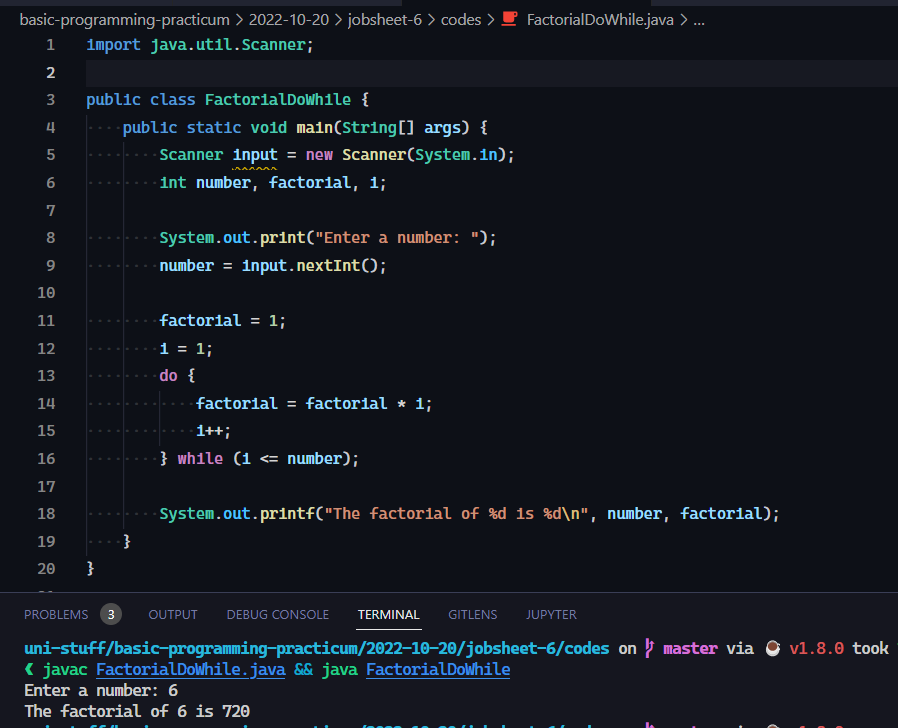
\includegraphics[width=.9\textwidth]{./images/factorial-do-while.png}
                    \caption{\texttt{FactorialDoWhile.java} final code and output}
                \end{figure}
            }
            \item {
                Match the results of the running programs that you have created according to the following display

                \begin{minted}[autogobble,fontsize=\small]{shell}
                    Enter a number: 6
                    The factorial of 6 is 720
                \end{minted}
            }
        \end{enumerate}
    }
\end{enumerate}
\pagebreak
\subsection{Experiment 2: Exit loop using break}
\begin{enumerate}
    \item Open a text editor. Create a new file, name it \textbf{LoopBreak.java}
    \item Write the basic structure of Java programming language which contains the \texttt{main()} function.
    \item Add the Scanner library
    \item Make a \textbf{Scanner} declaration with the name \texttt{input}
    \item Create multiple \texttt{int} type variables with names \texttt{number}, and \texttt{b}
    \item {
        Add the following code to enter the value from keyboard in 'for' loop structure.
        In 'for' loop there is also a condition to stop the process using the \texttt{break} statement.

        \begin{minted}[autogobble,fontsize=\small]{java}
            for (b = 0; true;) {
                System.out.print("Enter a number: ");
                number = input.nextInt();
                b += number;
                if (b > 50) {
                    break;
                }
            }
            System.out.printf("The numbers stop at the sum of the numbers %d\n", b);
        \end{minted}
    }
    \pagebreak
    \item {
        Compile and run the program. Observe the results!

        \begin{figure}[h]
            \centering
            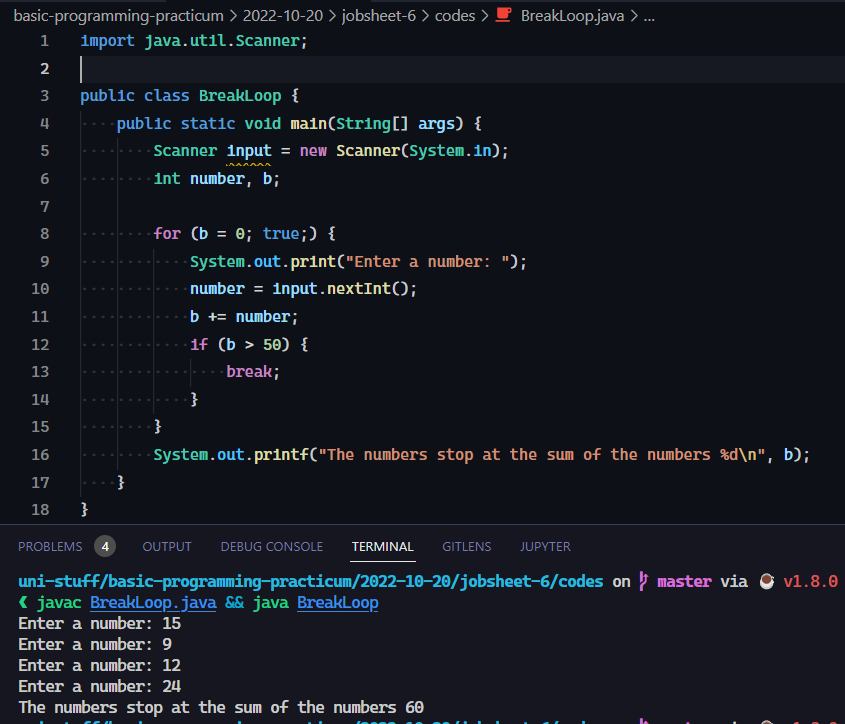
\includegraphics[width=.9\textwidth]{./images/break-loop.png}
            \caption{\texttt{BreakLoop.java} final code and output}
        \end{figure}
    }
    \item {
        Match the result of the running programs that you have created according to the following display

        \begin{minted}[autogobble,fontsize=\small]{shell}
            Enter a number: 15
            Enter a number: 9
            Enter a number: 12
            Enter a number: 24
            The numbers stop at the sum of the numbers 60
        \end{minted}
    }
\end{enumerate}

\pagebreak

\subsection{Experiment 3: Exit loop using continue}
\begin{enumerate}
    \item Open a text editor. Create a new file, name it \textbf{LoopBreak.java}
    \item Write the basic structure of Java programming language which contains the \texttt{main()} function.
    \item Add the Scanner library
    \item Make a \textbf{Scanner} declaration with the name \texttt{input}
    \item {
        Create multiple \texttt{int} type variables with names \texttt{number}, \texttt{b}, \texttt{i}, and \texttt{count}.
        Then also create two \texttt{double} type variables with names \texttt{avg} and \texttt{total}
    }
    \item {
        Add the following code to enter the value from keyboard in 'for' loop structure.
        In 'for' loop there is also a condition to stop the process using the \texttt{continue} statement.

        \begin{minted}[autogobble,fontsize=\small]{java}
            b = 0;
            count = 0;
            for (i = 0; i < 5; i++) {
                System.out.println("Enter a number: ");
                number = input.nextInt();
                if (number >= 50) {
                    continue;
                }
                b += number;
                count++;
            }
            total = (double) b;
            System.out.printf("The total number is less than 50: %.2f\n", total);
            avg = (double) b / count;
            System.out.printf("Average number less than 50: %.2f\n", avg);
        \end{minted}
    }
    \pagebreak
    \item {
        Compile and run the program. Observe the results!

        \begin{figure}[h]
            \centering
            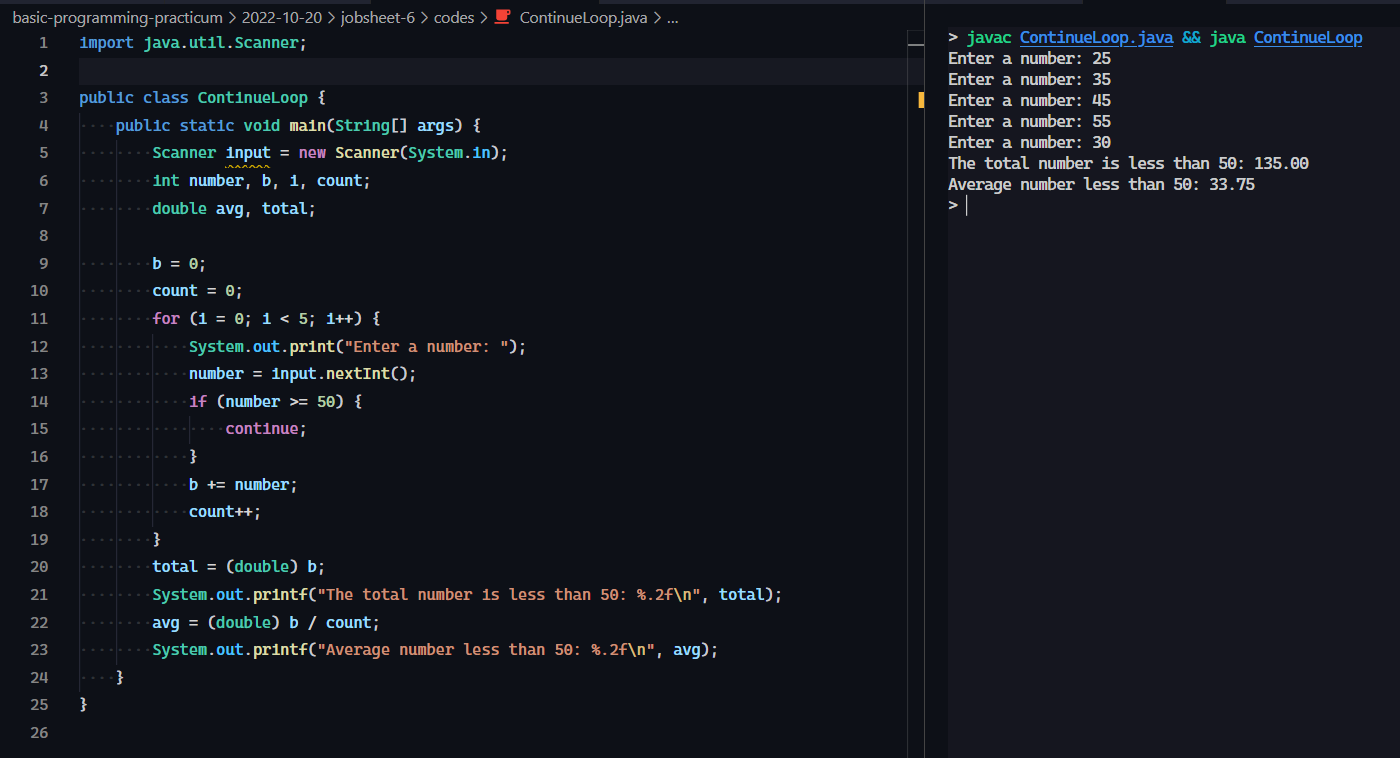
\includegraphics[width=.9\textwidth]{./images/continue-loop.png}
            \caption{\texttt{ContinueLoop.java} final code and output}
        \end{figure}
    }
    \item {
        Match the result of the running programs that you have created according to the following display

        \begin{minted}[autogobble,fontsize=\small]{shell}
            Enter a number: 25
            Enter a number: 35
            Enter a number: 45
            Enter a number: 55
            Enter a number: 30
            The total number is less than 50: 135.00
            Average number less than 50: 33.75
        \end{minted}
    }
\end{enumerate}

\pagebreak

\section{Questions!}
\begin{enumerate}
    \item {
        Explain the difference between Experiment 2 and Experiment 3!

        Experiment 2 uses the \texttt{break} keyword to stop the loop while Experiment 3 uses the \texttt{continue} keyword to stop the loop.
        The difference here is that the \texttt{break} keyword will 'break' out of the loop and it will \textit{stop} the loop without executing any of the code below of this keyword.
        The \texttt{continue} keyword will \textit{skip} the current iteration and 'continue' to the next iteration without executing the code below the keyword.
    }
    \item {
        Suppose you are asked to create a java program that asks for input of an integer \texttt{n}. Then the program displays the character '*' on the screen \textbf{n times}.
        Which of the two pieces of the program below is better and safer? Why?

        \begin{table*}[h]
            \centering
            \begin{tabular}{|p{.45\textwidth}|p{.45\textwidth}|}
                \hline
                \begin{minted}[autogobble,breaklines,fontsize=\small]{java}
                    /* for example: user input n has been stored in integer variable n */
                    int i = 0;

                    while (i < n) {
                        System.out.print("*");
                        i++;
                    }
                \end{minted}
                &
                \begin{minted}[autogobble,breaklines,fontsize=\small]{java}
                    /* for example: user input n has been stored in integer variable n */
                    int i = 0;

                    while (i != n) {
                        System.out.print("*");
                        i++;
                    }
                \end{minted}
                \\
                \hline
            \end{tabular}
        \end{table*}

        The first one (left) is better because it's more readable and its intent is more clear than the right one.
        We want the loop to run as long as \texttt{i} is less than \texttt{n} as opposed to \texttt{i} is not equal to \texttt{n}.
    }
    \pagebreak
    \item {
        What is the output of the following three code snippets?

        \begin{enumerate}[label=\alph*.]
            \item {
                \begin{minted}[autogobble,breaklines,fontsize=\small]{java}
                    int r = 1;
                    int i = 1;
                    int a = 2;
                    int n = 4;
        
                    while (i <= n) {
                        r = r * a;
                        i++;
                    }
        
                    System.out.print(r);
                \end{minted}

                The output of the code above is \texttt{6}
            }
            \item {
                \begin{minted}[autogobble,breaklines,fontsize=\small]{java}
                    int n = 5;
                    boolean stop = false;
        
                    int i = 1;
                    while (!stop) {
                        if (i >= n) {
                            stop = true;
                        } else {
                            if (i % 2 == 1) {
                                System.out.println("#");
                            } else {
                                System.out.println("*");
                            }
                        }
                        i++;
                    }
                \end{minted}

                The output of the code above is:

                \begin{minted}[autogobble,fontsize=\small]{shell}
                    #
                    *
                    #
                    *
                \end{minted}
            }
            \item {
                \begin{minted}[autogobble,breaklines,fontsize=\small]{java}
                    int n = 5;
                    long result = 1;
                    for (int i = 1; i <= n; i++) {
                        result = result * i;
                    }
                    System.out.println(n + "!=" + result);
                \end{minted}

                The output of the code above is: \texttt{5!=120}
            }
        \end{enumerate}
    }
\end{enumerate}

\pagebreak

\section{Assignment}
\begin{enumerate}
    \item {
        Create a program to display numbers from 1 to the user input numbers sequentially and skip the multiples of 5 as shown below!

        \begin{multicols}{2}
            \begin{minted}[autogobble,fontsize=\small]{shell}
                Enter a number: 12
                1
                2
                3
                4
                6
                7
                8
                9
                11
                12
            \end{minted}
            \columnbreak
            \begin{minted}[autogobble,fontsize=\small]{shell}
                Enter a number: 9
                1
                2
                3
                4
                6
                7
                8
                9
            \end{minted}
        \end{multicols}

        \begin{figure}[h]
            \centering
            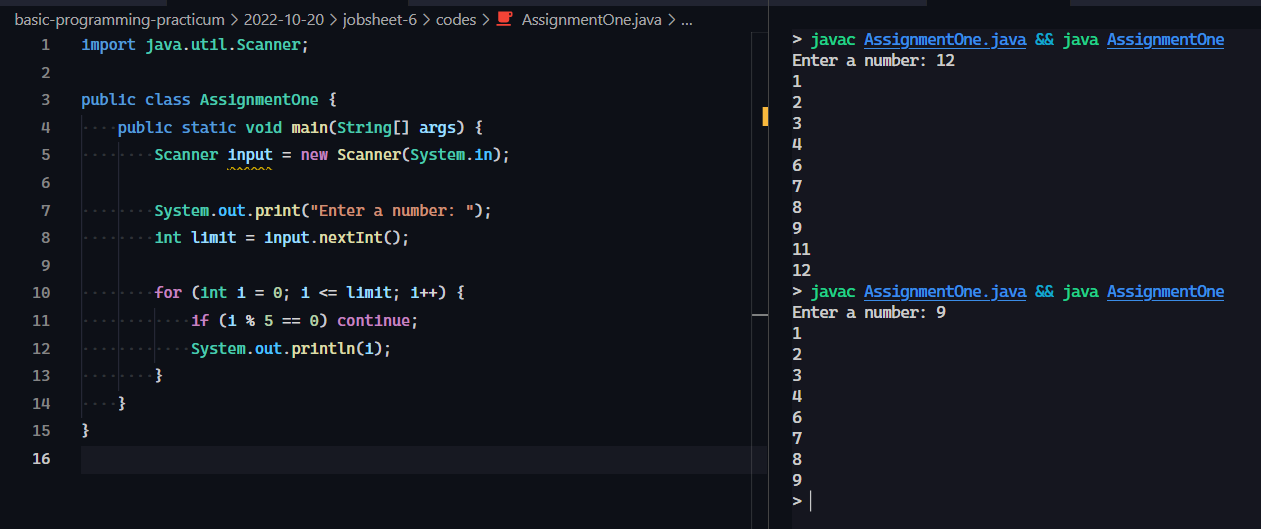
\includegraphics[width=.9\textwidth]{./images/assignment-one.png}
            \caption{\texttt{AssignmentOne.java} final code and output}
        \end{figure}
    }
    \item {
        Create a program using the Java programming language that requests input of an integer N (N$>$0) from user.
        The program then displays the sum of \textbf{the first N positive even numbers (even numbers $\geq$ 0)}.

        Example:
        \begin{itemize}
            \item {
                If the user enters N = 10, the program will count the number of positive numbers in the range 1-10 then display the sum of
                positive numbers between 1-10, namely:
                \[
                    0 + 2 + 4 + 6 + 8 + 10 = 30
                \]
                After that the program will display the average of the positive numbers that were added earlier.
            }
            \item {
                Example of program output

                \begin{minted}[autogobble,fontsize=\small]{shell}
                    Enter a number range: 10
                    The number of even numbers from 1 to 10 is 5
                    Even number 1 is 2
                    Even number 2 is 4
                    Even number 3 is 6
                    Even number 4 is 8
                    Even number 5 is 10
                    The sum of the even numbers from 1 to 10 is 30
                    The average of the even numbers from 1 to 10 is 6.00
                \end{minted}

                You can design your own for the program display
            }
        \end{itemize}

        \begin{figure}[h]
            \centering
            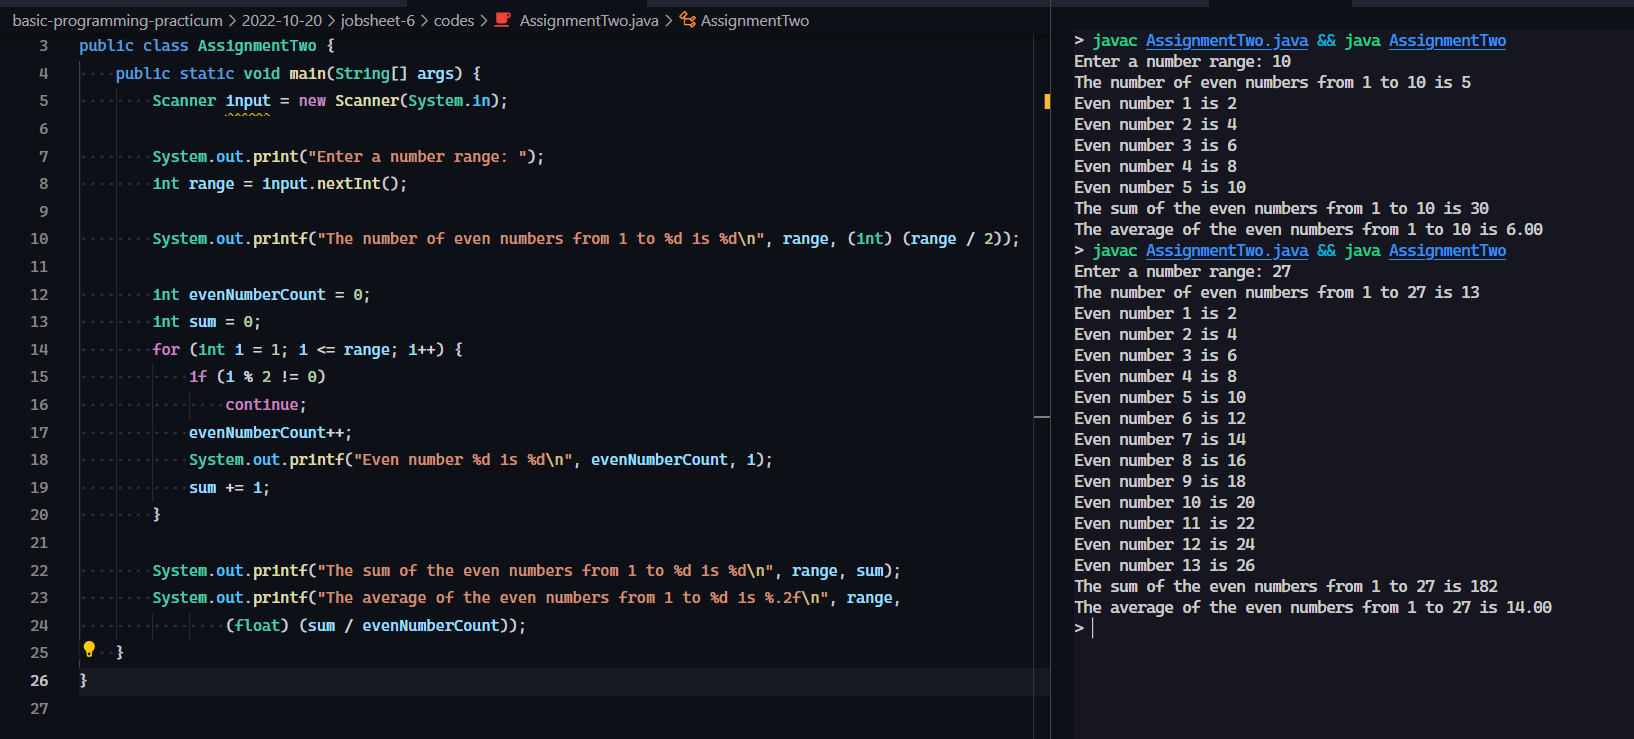
\includegraphics[width=.9\textwidth]{./images/assignment-two.png}
            \caption{\texttt{AssignmentTwo.java} final code and output}
        \end{figure}
    }
\end{enumerate}

\end{document}

